
\documentclass[letterpaper,11pt,leqno]{article}
\usepackage{paper}

% Enter paper title to populate PDF metadata:
\hypersetup{pdftitle={Relazione di Progetto: Parallelizzazione dell'algoritmo Skyline}}

% Enter path to PDF file with figures:
\newcommand{\pdf}{figures.pdf}

% Custom title definition
\title{\vspace{-1cm} Relazione di progetto \\ Corso di High Performance Computing \\ A.A. 2024-2025}
\author{Alessandro Valmori}
\date{\vspace{-0.5cm} \today}  % Adjust space before the date

\begin{document}

\begingroup\let\newpage\relax\maketitle\endgroup  % Removes forced page break

\vspace{-1cm}  % Adjust spacing after the title





% Enter main text:
\section{Introduzione}\label{s:introduction}
 
Si sceglie di implementare la parallelizazione dell'algoritmo Skyline in due diverse versioni, utilizzando prima OpenMP e poi MPI, due tecniche di parallelizzazione rispettivamente a memoria condivisa e a memoria distribuita. L'approccio alla parallelizzazione utilizzando i due paradigmi condivide la fase di partizionamento del dominio iniziale fra i processi, utilizzando in particolare un partizionamento statico a grana grossa. 



\section{Versione OpenMP}\label{s:section}


Per la versione a memoria condivisa utilizzando OpenMP, si sceglie di parallellizzare il confronto fra un punto e tutti gli altri. In particolare il ciclo esterno, che itera attraverso i punti da esaminare, è stato parallellizzato utilizzando la direttiva \texttt{\#pragma omp parallel for}. Per calcolare il numero di punti nello skyline set (l'insieme di punti non dominati), è stato applicato il pattern di riduzione. Nella riduzione, il valore di \texttt{r} (il contatore che tiene traccia dei punti nello skyline) viene modificato da più thread senza conflitti grazie alla direttiva \texttt{reduction(-:r)}. Ogni volta che un punto è trovato dominante su un altro, il punto dominante viene segnato come non appartenente allo skyline (modificando l'array \texttt{s}), e il contatore \texttt{r} viene decrementato. Per evitare il controllo ripetuto di punti già rimossi dallo skyline, ogni punto viene esaminato una sola volta, e non appena si trova un punto che domina un altro, quest'ultimo viene rimosso.


\begin{figure}[h]
  \centering
    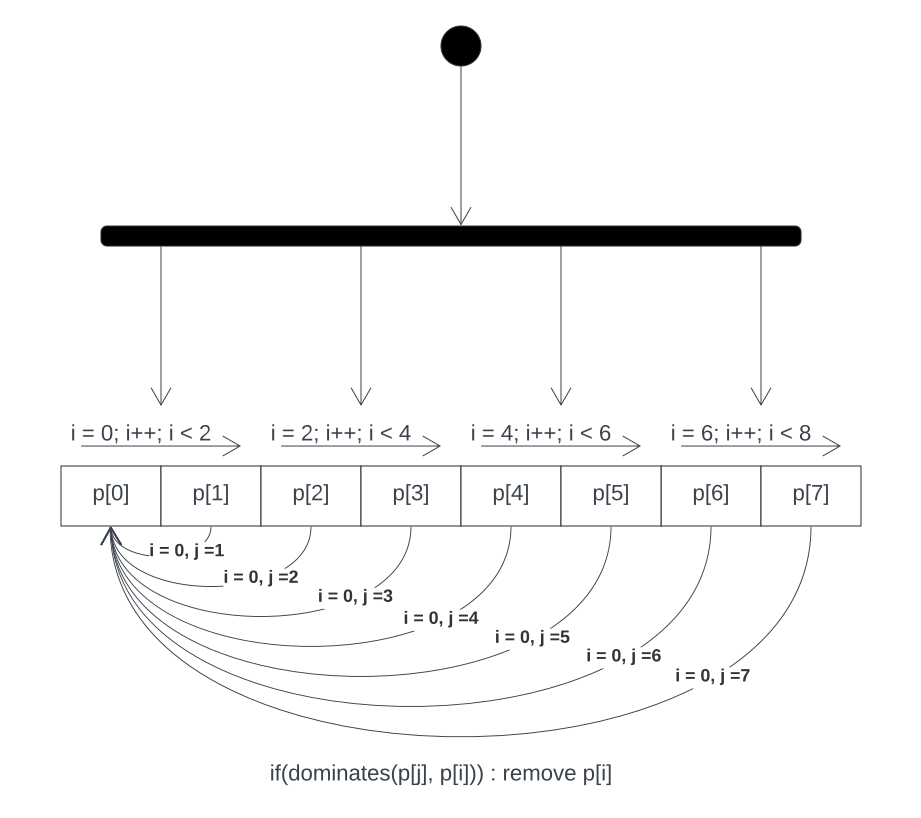
\includegraphics[scale=0.4]{OMP.pdf}
    \caption{Schema concettuale del processo svolto dall'algoritmo parallelo con OpenMP}
    \label{f:graph1}
\end{figure}







\section{Versione MPI}\label{s:section}


Per la versione a memoria distribuita utilizzando MPI è stata implementata una soluzione che presenta un processo più scandito e verboso, che comincia con la suddivisione del dominio iniziale in parti il quanto più possibile eguali fra i processi. Questo partizionamento avviene staticamente e grossolanamente dopo che il processo \texttt{master} ha letto l’insieme di punti da standard input.

Una volta che ciascun processo detiene la propria partizione dell’input set originale, ognuno di essi applica la versione seriale dell’algoritmo Skyline a quest’ultima, ottenendo quindi un sottoinsieme di tale partizione costituito dai punti che non sono dominati da alcun altro punto all’interno della partizione.

In seguito, il processo \texttt{master} esegue una \texttt{MPI\_Gatherv} di ciascuno skyline set locale in un unico array, di cui ne viene poi distribuita una copia a ciascun processo, in modo da consentire il confronto fra lo skyline set locale e tale array. Infine, dopo che ciascun processo ha rimosso dalla propria partizione tutti i punti dominati, avviene una chiamata alla funzione \texttt{MPI\_Reduce} per ottenere il numero totale di punti presenti nello skyline finale, seguita da un’ulteriore chiamata a \texttt{MPI\_Gatherv} per concatenare tutti i singoli array locali nello skyline finale.

\begin{figure}[h]
    \centering
    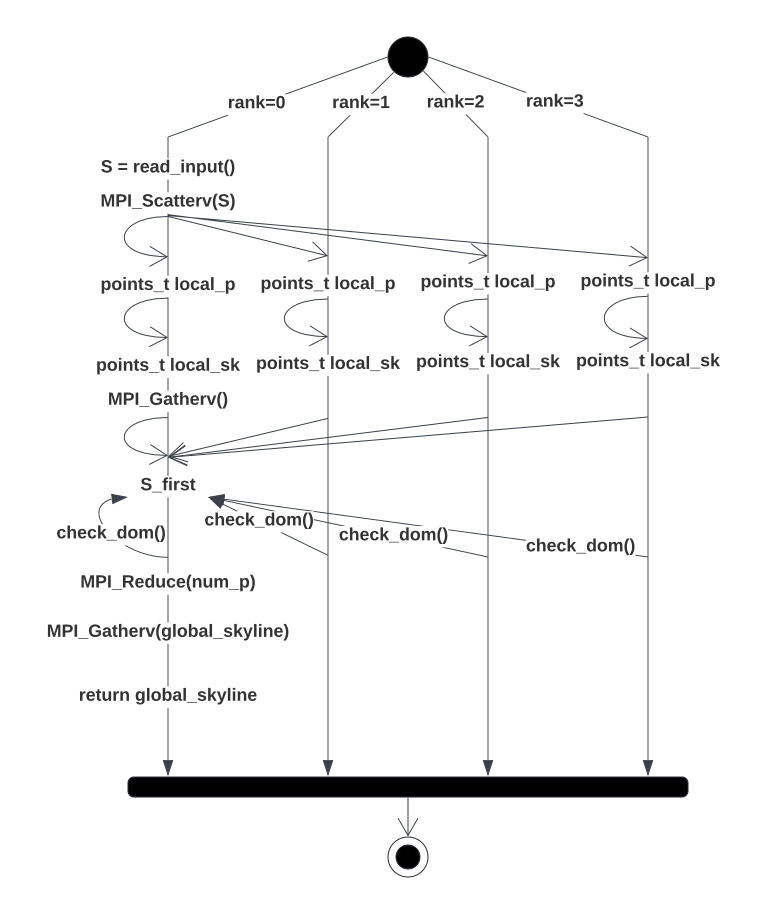
\includegraphics[scale=0.6]{MPI.pdf}
    \caption{Schema concettuale del processo svolto dall'algoritmo parallelo con MPI}
    \label{f:graph2}
\end{figure}




\section{Prestazioni}

Per valutare l'efficacia dell'implementazione parallela dell'algoritmo Skyline, sono stati condotti test mirati all'analisi dello Strong Scaling e del Weak Scaling. L'obiettivo è verificare come il tempo di esecuzione varia al variare del numero di processi, sia mantenendo fisso il carico di lavoro totale (Strong Scaling) sia mantenendo costante il carico per processo (Weak Scaling).  

I test sono stati eseguiti su una macchina con processore Intel Core i7-1165G7 di undicesima generazione (4 core fisici, 8 thread) e 16GB di RAM. L'algoritmo è stato eseguito 10 volte per ciascuna configurazione sperimentale, e il valore finale riportato corrisponde alla media dei tempi di esecuzione ottenuti, riducendo così l'effetto di eventuali variazioni dovute a fattori esterni, come il sistema operativo o altri processi in esecuzione.  

Per raccogliere i dati, è stato realizzato uno script bash che automatizza l'esecuzione delle prove. Lo script si occupa di lanciare il programma con diverse configurazioni di numero di processi MPI e dataset di input, redirezionando l'output standard e gli errori in un file di log per facilitare l'analisi successiva. Inoltre, un insieme di script Python è stato utilizzato per elaborare i risultati e generare grafici rappresentativi delle prestazioni ottenute.  

\subsection{Strong Scaling}

Durante la valutazione dello Strong Scaling si analizza il comportamento dell'algoritmo mantenendo costante la dimensione del problema e aumentando progressivamente il numero di processi utilizzati per l'esecuzione. L'obiettivo è osservare come varia il tempo di esecuzione e verificare se l'algoritmo è in grado di sfruttare in modo efficiente un numero crescente di processi.  

Per questi test, è stato scelto un dataset di dimensione fissa, ovvero 50000 punti di 20 dimensioni dapprima costituenti uno Skyline set valido, rappresentativo di un caso d'uso realistico che corrisponde anche al caso pessimo. Il numero di processi è stato variato da 1 a 8, in modo da valutare il comportamento dell'algoritmo sia in condizioni di esecuzione seriale (1 processo) sia quando si sfruttano tutte le risorse disponibili sulla macchina di test (8 processi, pari al numero massimo di thread del processore).  

Idealmente, in uno scenario di perfetto Strong Scaling, il tempo di esecuzione dovrebbe ridursi proporzionalmente all'aumento del numero di processi. Tuttavia, in una situazione reale, il comportamento può essere influenzato da diversi fattori, tra cui l'overhead della comunicazione tra processi, il bilanciamento del carico e le latenze introdotte dalla gestione della memoria. 


\begin{figure}[h]
    \centering
    \begin{subfigure}{0.48\textwidth} % Prima immagine occupa il 48% della larghezza
        \centering
        \includegraphics[scale=0.3]{graphs/omp_strong_scaling.pdf}
        \caption{Tempo di esecuzione in funzione del numero di processi (Strong Scaling) di OpenMP}
        \label{f:strong_scaling}
    \end{subfigure}
    \hfill % Aggiunge spazio tra le due immagini
    \begin{subfigure}{0.48\textwidth} % Seconda immagine
        \centering
        \includegraphics[scale=0.3]{graphs/mpi_strong_scaling.pdf}
        \caption{Tempo di esecuzione in funzione del numero di processi (Strong Scaling) di MPI}
        \label{f:strong_scaling_speedup}
    \end{subfigure}
    \caption{Analisi dello strong scaling dell'algoritmo}
    \label{f:strong_scaling_graphs}
\end{figure}
  


\subsection{Weak Scaling}

Il Weak Scaling valuta come varia il tempo di esecuzione dell'algoritmo quando sia il numero di processi (o thread) che la dimensione del problema aumentano. L'obiettivo è determinare se l'efficienza parallela rimane stabile con l'aggiunta di risorse computazionali.

\subsubsection{Metodologia di Scalabilità}
La complessità parallela dell'algoritmo skyline può essere espressa come:

\[
O\left(\frac{N^2 D}{p}\right)
\]

dove:
\begin{itemize}
    \item \( N \) = numero di punti,
    \item \( D \) = numero di dimensioni (assunto costante),
    \item \( p \) = numero di processi (o thread).
\end{itemize}

Ogni thread è responsabile di un sottoinsieme dei confronti totali \( N^2 \), dato da:

\[
\frac{N^2}{p}
\]

Per mantenere il carico di lavoro per processo costante, dobbiamo garantire che questo termine rimanga invariato all'aumentare di \( p \). Ciò porta alla condizione:

\[
\frac{(N')^2}{p'} = \frac{N^2}{p}
\]

dove:
\begin{itemize}
    \item \( N' \) è la nuova dimensione del problema con \( p' \) thread,
    \item \( N \) è la dimensione originale con \( p \) thread.
\end{itemize}

\subsubsection{Derivazione del Fattore di Scalabilità}
Riorganizzando la formula per \( N' \), otteniamo:

\[
N' = N \times \sqrt{\frac{p'}{p}}
\]

Questo significa che, per mantenere il carico di lavoro per processo costante, la dimensione del problema \( N \) deve essere aumentata di un fattore:

\[
\sqrt{p}
\]


\subsubsection{Risultati Sperimentali}
Per analizzare il Weak Scaling, si sono eseguiti test in cui sia il numero di thread \( p \) che la dimensione del dataset \( N \) sono stati aumentati secondo la regola di scalabilità derivata sopra.

\begin{figure}[h]
    \centering
    \begin{subfigure}{0.48\textwidth}
        \centering
        \includegraphics[scale=0.3]{graphs/omp_weak_scaling.pdf}
        \caption{Risultati del Weak Scaling con OpenMP.}
        \label{f:weak_scaling_omp}
    \end{subfigure}
    \hfill
    \begin{subfigure}{0.48\textwidth}
        \centering
        \includegraphics[scale=0.3]{graphs/mpi_weak_scaling.pdf}
        \caption{Risultati del Weak Scaling con MPI.}
        \label{f:weak_scaling_mpi}
    \end{subfigure}
    \caption{Analisi del Weak Scaling per le implementazioni OpenMP e MPI.}
    \label{f:weak_scaling_graphs}
\end{figure}

I risultati in Figura \ref{f:weak_scaling_graphs} mostrano che:
\begin{itemize}
    \item OpenMP: Il tempo di esecuzione rimane relativamente stabile per un numero ridotto di thread, ma aumenta con valori più elevati a causa dell'overhead di sincronizzazione e della contesa della memoria condivisa.
    \item MPI: La performance scala meglio inizialmente, ma l'overhead di comunicazione diventa significativo all'aumentare del numero di processi.
\end{itemize}

In uno scenario ideale di Weak Scaling, il tempo di esecuzione dovrebbe rimanere costante con l'aumento simultaneo della dimensione del problema e delle risorse computazionali. Tuttavia, limitazioni reali come contesa della memoria, overhead di comunicazione e squilibri nel bilanciamento del carico contribuiscono a deviazioni da questo comportamento ideale.


\subsection{Speedup}

I risultati sperimentali per lo strong scaling sono stati elaborati per ottenere lo speedup e l'efficienza per ciascun numero di processori. I calcoli sono stati effettuati utilizzando la formula:
\[
\text{Speedup}(p) = \frac{T(1)}{T(p)} \quad\text{e}\quad \text{Efficienza}(p) = \frac{\text{Speedup}(p)}{p},
\]
dove \(T(1)\) è il tempo medio di esecuzione su 1 processore e \(T(p)\) è il tempo medio di esecuzione su \(p\) processori.

Di seguito vengono riportate due tabelle riassuntive (con valori espressi in secondi per \(T(p)\)):



\begin{table}[htbp]
\centering
\caption{Speedup e Efficienza per lo Strong Scaling: confronto tra OpenMP e MPI}
\label{tab:combined_speedup}
\adjustbox{max width=\textwidth}{%
\begin{tabular}{cc}
    \begin{subtable}{0.48\textwidth}
        \centering
        \caption{OpenMP}
        \label{tab:openmp_speedup}
        \footnotesize % or \scriptsize if needed
        \setlength{\tabcolsep}{3pt} % Reduce horizontal spacing
        \begin{tabular}{cccc}
        \toprule
        N. Proc & \(T(p)\) (s) & Speedup & Efficienza\\
        \midrule
        1 & 0.139875 & 1.000 & 1.000\\
        2 & 0.086947 & 1.609 & 0.804\\
        3 & 0.065455 & 2.137 & 0.712\\
        4 & 0.048127 & 2.906 & 0.727\\
        5 & 0.040795 & 3.429 & 0.686\\
        6 & 0.034562 & 4.047 & 0.675\\
        7 & 0.034850 & 4.014 & 0.573\\
        8 & 0.036928 & 3.788 & 0.473\\
        \bottomrule
        \end{tabular}
    \end{subtable} &
    \begin{subtable}{0.48\textwidth}
        \centering
        \caption{MPI}
        \label{tab:mpi_speedup}
        \footnotesize % or \scriptsize if needed
        \setlength{\tabcolsep}{3pt} % Reduce horizontal spacing
        \begin{tabular}{cccc}
        \toprule
        N. Proc & \(T(p)\) (s) & Speedup & Efficienza\\
        \midrule
        1 & 0.120000 & 1.000 & 1.000\\
        2 & 0.080000 & 1.500 & 0.750\\
        3 & 0.070000 & 1.714 & 0.571\\
        4 & 0.050000 & 2.400 & 0.600\\
        5 & 0.045000 & 2.667 & 0.533\\
        6 & 0.040000 & 3.000 & 0.500\\
        7 & 0.038000 & 3.158 & 0.451\\
        8 & 0.035000 & 3.429 & 0.429\\
        \bottomrule
        \end{tabular}
    \end{subtable}
\end{tabular}%
}
\end{table}




\section{Conclusioni}






\end{document}
